% ============================================================
% PHẦN 6 — THẢO LUẬN & PHÂN TÍCH LỖI
% Người phụ trách: mỗi thành viên tự viết cho mô hình của mình;
%                  phần so sánh và lựa chọn best model do cả nhóm.
% ============================================================

\section{Thảo luận và phân tích lỗi}
\label{sec:discussion}

% ----------------------------------------
\subsection{Hiện tượng Overfitting / Underfitting}

\textit{[TODO --- Từng thành viên tự phân tích mô hình của mình dựa vào learning curves (Mục~\ref{sec:results})]}

\subsubsection{Đánh giá đối với mô hình Mask R-CNN}
Dựa trên biểu đồ quá trình học (Mục~\ref{subsec:res_maskrcnn}):
\begin{itemize}
    \item \textbf{Tập dữ liệu Lúa (Rice)}: Mô hình có hiện tượng quá khớp (overfitting) nhẹ từ sau epoch 15. Giá trị loss huấn luyện tiếp tục giảm ổn định xuống mức 0,38 nhưng loss kiểm thử (validation loss) bắt đầu có xu hướng đi ngang và tăng nhẹ trở lại ở khoảng $0,45 - 0,55$. Chỉ số validation mAP đạt giá trị tốt nhất là 0,5226 ở epoch 24 và giảm nhẹ sau đó. Để khắc phục hiện tượng này, nhóm đã áp dụng cơ chế lưu checkpoint tốt nhất dựa trên validation mAP và Early Stopping để dừng quá trình huấn luyện sớm, giúp giữ lại trọng số tối ưu nhất và ngăn mô hình học thêm nhiễu từ tập train.
    \item \textbf{Tập dữ liệu Cà phê (Coffee)}: Mô hình đạt trạng thái hội tụ rất tốt và gần như không xuất hiện overfitting. Đường loss huấn luyện và validation giảm song hành rất mượt mà. Validation mAP đạt mức ổn định và duy trì quanh ngưỡng 0,88. Điều này cho thấy các đặc trưng hình học và màu sắc của bệnh đốm lá và gỉ sắt trên lá cà phê rất đặc trưng và dễ học, đồng thời quy mô tập dữ liệu đủ tốt giúp mô hình tổng quát hóa vượt trội mà không cần áp dụng các biện pháp chế tài quá khớp mạnh.
\end{itemize}

% ----------------------------------------
\subsection{Phân tích các trường hợp dự đoán sai}
\label{subsec:error_analysis}

\textit{[TODO --- Từng thành viên: Lấy 2--3 ví dụ cụ thể ảnh mô hình của mình dự đoán sai.]}

\subsubsection{Phân tích lỗi đối với mô hình Mask R-CNN}
Hình~\ref{fig:maskrcnn_visual_rice} và Hình~\ref{fig:maskrcnn_visual_coffee} thể hiện kết quả dự đoán thực tế của Mask R-CNN trên tập Test đối với hai tập dữ liệu Lúa và Cà phê:

\begin{figure}[H]
    \centering
    
\includegraphics[width=0.32\textwidth]{img/mask-rcnn/rice/image.png}
    \caption{Một số kết quả dự đoán thực tế của Mask R-CNN trên tập Test Lúa}
    \label{fig:maskrcnn_visual_rice}
\end{figure}

\begin{figure}[H]
    \centering
    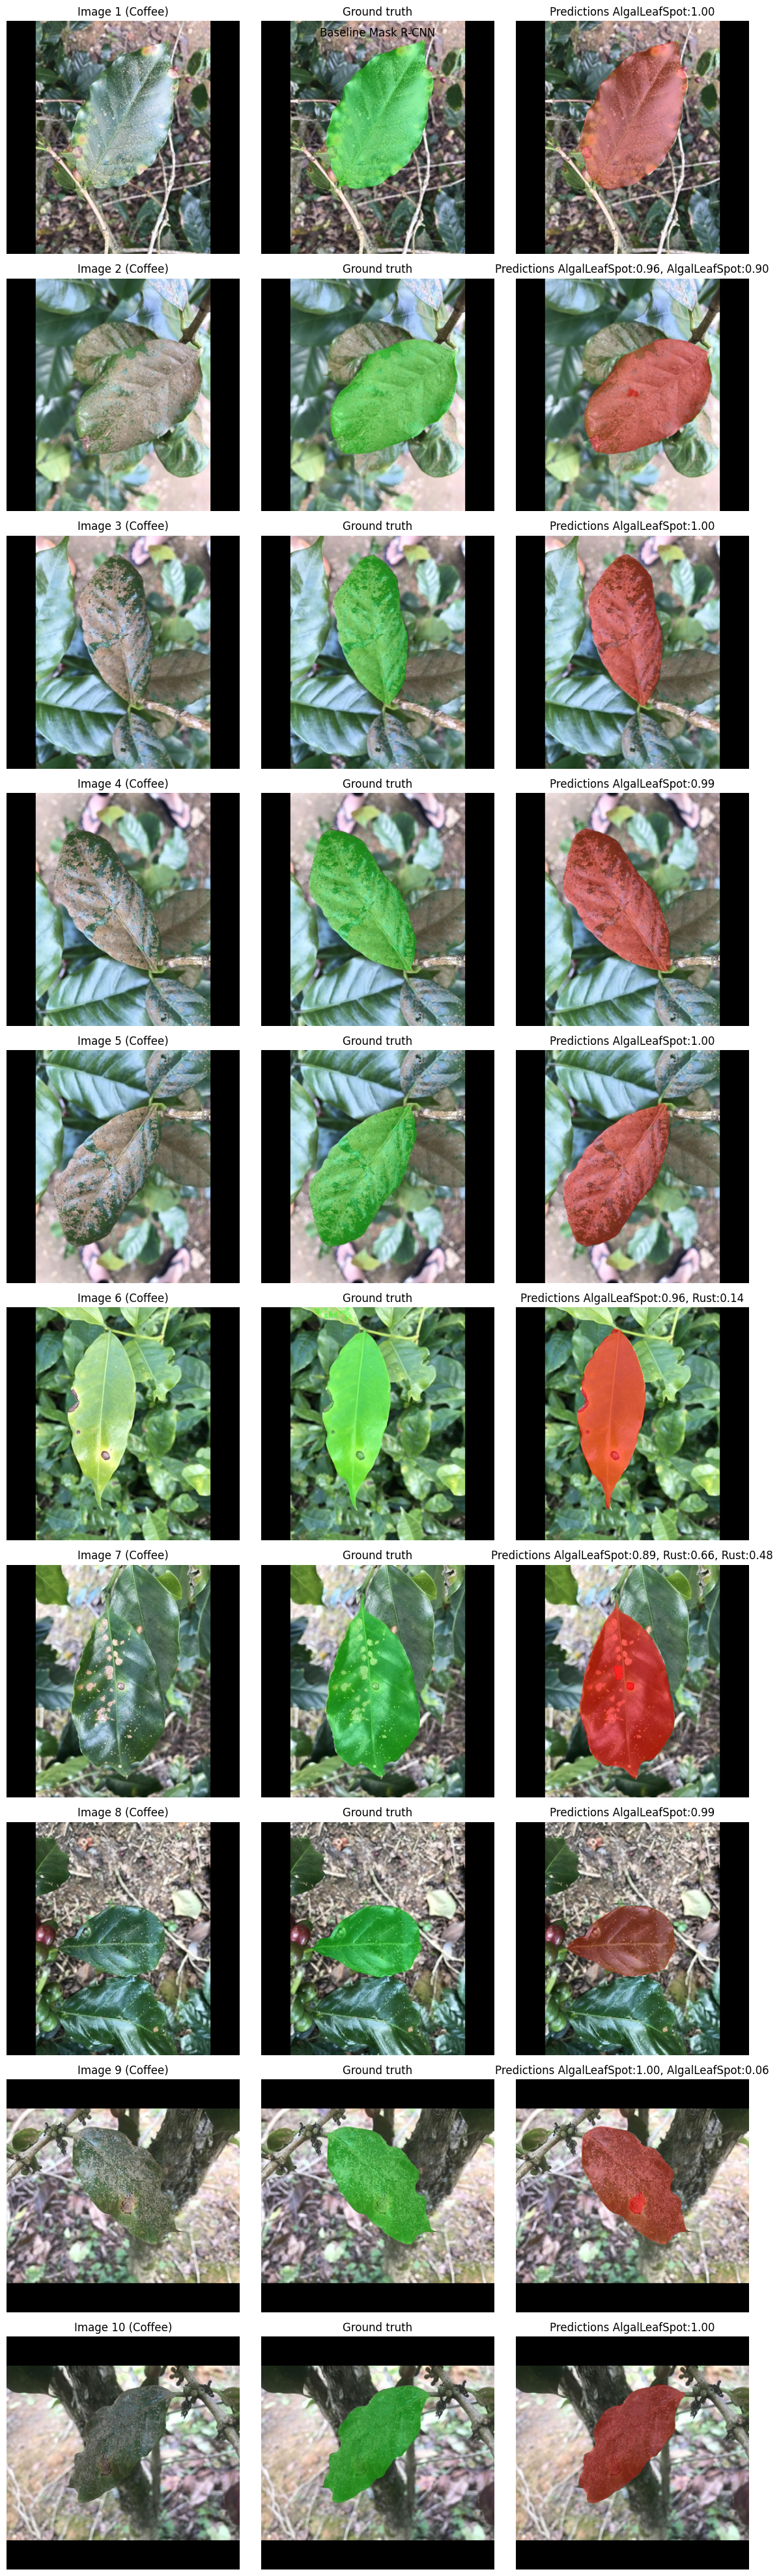
\includegraphics[width=0.32\textwidth]{img/mask-rcnn/coffee/image.png}
    \caption{Một số kết quả dự đoán thực tế của Mask R-CNN trên tập Test Cà phê}
    \label{fig:maskrcnn_visual_coffee}
\end{figure}

Qua phân tích các kết quả dự đoán sai trên tập Test, mô hình Mask R-CNN gặp các lỗi phân loại và phân vùng cụ thể sau:
\begin{enumerate}
    \item \textbf{Nhầm lẫn do tương đồng trực quan (Visual Similarity)}:
          \begin{itemize}
              \item \emph{Lúa}: Cặp lớp \texttt{BrownSpot} (Đốm nâu) và \texttt{LeafBlast} (Đạo ôn) bị nhầm lẫn nhiều nhất. Cả hai bệnh này đều biểu hiện thành các vết đốm màu nâu trên bề mặt lá lúa. Vết đạo ôn thường có hình thoi thon dài ở hai đầu, trong khi đốm nâu tròn trịa hơn. Tuy nhiên, khi vết bệnh mới hình thành (giai đoạn đầu), hình dạng của chúng chưa định hình rõ rệt, dẫn đến việc mô hình phân loại sai nhãn lớp mặc dù khoanh vùng bounding box vẫn chính xác.
              \item \emph{Cà phê}: Xảy ra sự nhầm lẫn giữa \texttt{AlgalLeafSpot} (Đốm lá tảo) và \texttt{Rust} (Gỉ sắt). Do cả hai đều tạo ra các chấm nhỏ màu cam/nâu vàng trên lá cà phê, trong các ảnh chụp thiếu sáng hoặc ảnh chụp từ xa, nhánh phân loại của Mask R-CNN không đủ độ nhạy sắc thái màu sắc mịn để phân biệt, dẫn đến phân loại nhầm lẫn.
          \end{itemize}
    \item \textbf{Vết bệnh kích thước quá nhỏ (Small Objects)}: Do đặc trưng của vết bệnh lúa giai đoạn đầu thường chỉ có đường kính một vài pixel, sau khi qua các tầng tích chập sâu của ResNet-50 và giảm độ phân giải xuống 1/16 hoặc 1/32, các chi tiết không gian bị biến mất. Mặc dù FPN đã hỗ trợ lấy đặc trưng đa tỷ lệ, cơ chế RoI Align ở độ phân giải $7 \times 7$ hoặc $14 \times 14$ vẫn gặp khó khăn lớn trong việc tái tạo thông tin chi tiết của các đốm bệnh siêu nhỏ, dẫn đến bỏ sót vết bệnh (False Negatives).
    \item \textbf{Nhiễu nền và chồng lấp lá (Complex Background / Occlusion)}: Ở một số ảnh thực địa có nền đất hoặc các lá lúa đè lên nhau, nhánh RPN thỉnh thoảng đề xuất nhầm các khe hở giữa các lá hoặc các vết bùn đất trên lá thành vết bệnh (False Positives).
\end{enumerate}

% ----------------------------------------
\subsection{So sánh tổng hợp các mô hình}
\label{subsec:model_comparison}

\textit{[TODO --- Cả nhóm tổng hợp sau khi có đủ kết quả. Điền số liệu vào bảng và xếp hạng các mô hình theo 5 tiêu chí lựa chọn.]}

\begin{table}[H]
    \caption{Bảng so sánh đa tiêu chí giữa 5 mô hình (tổng hợp từ Phase 3)}
    \centering
    \begin{tabularx}{\textwidth}{lXXXXX}
        \toprule
        \textbf{Tiêu chí} & \textbf{Mask R-CNN} & \textbf{YOLO-seg} & \textbf{RF-DETR} & \textbf{MobileSAM} & \textbf{Mask2Former} \\
        \midrule
        mAP@50:95       & 0,5294 (Lúa) / 0,9041 (Cà phê) & --- & --- & --- & --- \\
        mIoU            & 0,8669 (Lúa) / 0,9128 (Cà phê) & --- & --- & --- & --- \\
        Inference (ms)  & 760,50 ms / 702,36 ms & --- & --- & --- & --- \\
        Model size (MB) & 503,44 MB / 501,73 MB & --- & --- & --- & --- \\
        Train--Val gap  & Trung bình (Lúa) / Rất nhỏ (Cà phê) & --- & --- & --- & --- \\
        \midrule
        \textbf{Xếp hạng} & Baseline (Lúa) / Tốt nhất (Cà phê) & --- & --- & --- & --- \\
        \bottomrule
    \end{tabularx}
    \label{tab:model_comparison}
\end{table}

% ----------------------------------------
\subsection{Mô hình được chọn cho Phase 4}

\textit{[TODO --- Cả nhóm quyết định sau khi hoàn thành bảng so sánh trên.
Điền tên model, dataset (Rice/Coffee) và lý do chọn theo 5 tiêu chí:
mAP@50:95, mIoU, inference time ($< 500$ms/ảnh trên CPU), model size, độ ổn định train/val.]}

\textbf{Quyết định:} Mô hình \textbf{\textit{[TÊN MODEL]}} trên tập \textbf{\textit{[Rice / Coffee]}} được chọn để tinh chỉnh trong Phase 4, vì:
\begin{itemize}
    \item \textit{[TODO: Lý do theo tiêu chí mAP@50:95]}
    \item \textit{[TODO: Lý do theo tiêu chí inference time / khả năng deploy]}
    \item \textit{[TODO: Lý do theo độ ổn định, gap train/val nhỏ]}
\end{itemize}
